\section{Resultados}

\subsection*{Experimento 1}
Utilizando a rede RBF com regularização foi realizado um problema de classificação com os pacotes de dados make circles e make moons disponíveis no repositório sklearn. \footcite{https://scikit-learn.org/stable/}

\begin{figure}[H]
    \center
    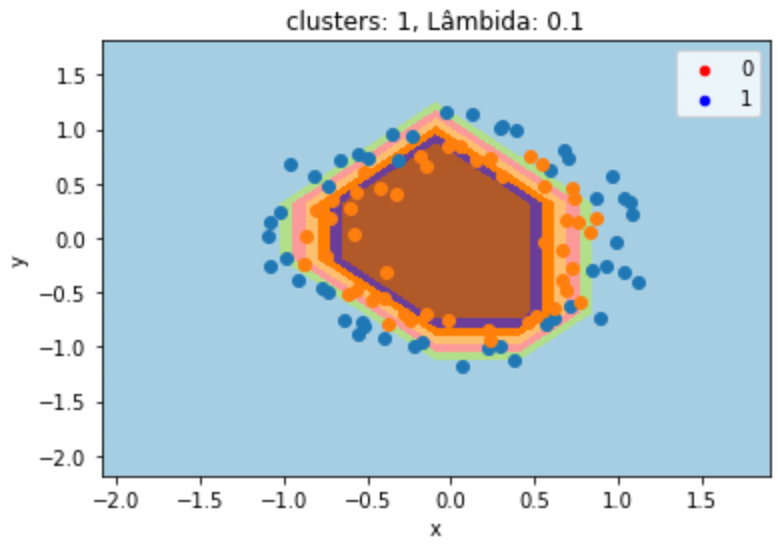
\includegraphics[width=6cm]{images/img1.png}
    \caption{\label{img1}RBF: 1 cluster e regularização = 0.1}
  \end{figure}

  \begin{figure}[H]
    \center
    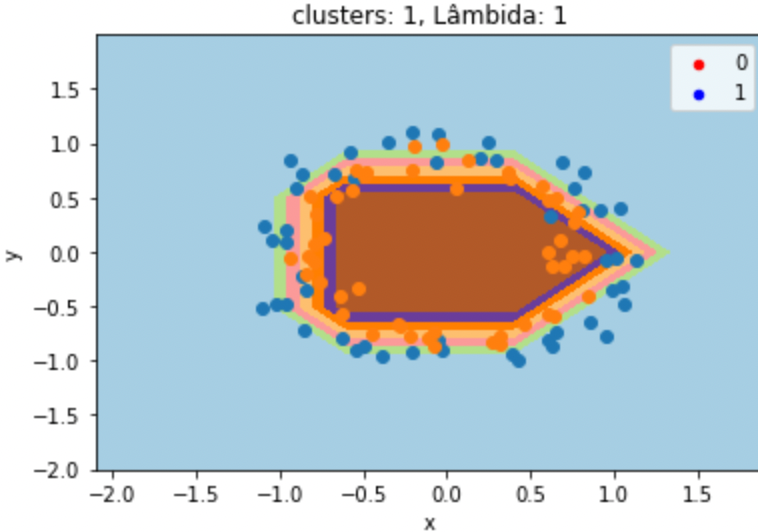
\includegraphics[width=6cm]{images/img2.png}
    \caption{\label{img2}RBF: 1 cluster e regularização = 1}
  \end{figure}

  \begin{figure}[H]
    \center
    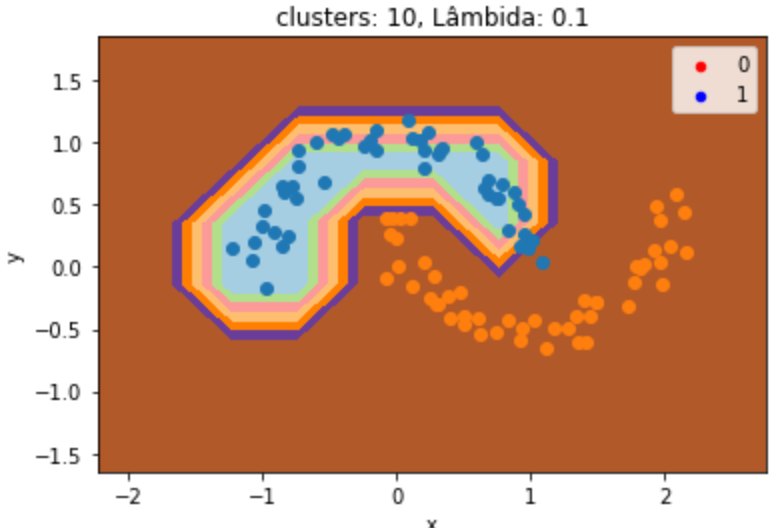
\includegraphics[width=6cm]{images/img3.png}
    \caption{\label{img3}RBF: 10 cluster e regularização = 0.1}
  \end{figure}

  \begin{figure}[H]
    \center
    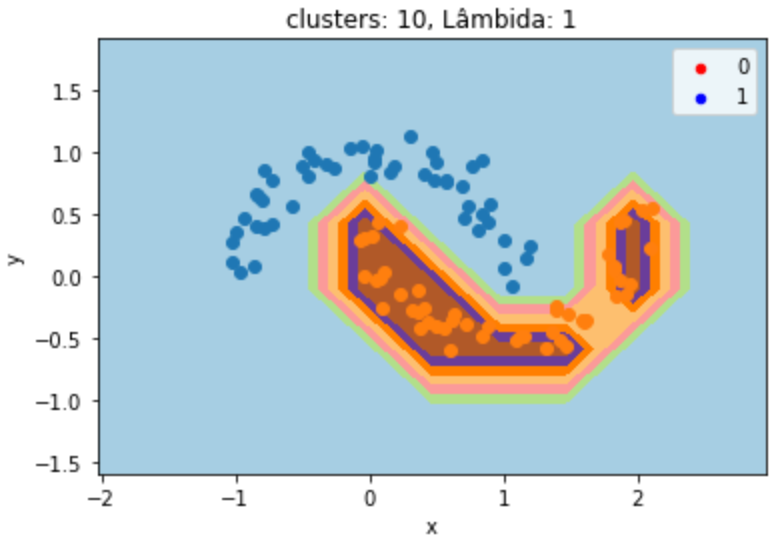
\includegraphics[width=6cm]{images/img4.png}
    \caption{\label{img4}RBF: 10 cluster e regularização = 1}
  \end{figure}

Nesse experimento a quantidade de clusters foi escolhida por meio de testes de forma a gerar o melhor resultado para cada base de dados selecionada. Como o objetivo é avaliar
o efeito da regularização, a quantidade de clusters se manteu fixo.




\subsection*{Experimento 2}

Esse experimento foi realizado utilizando a base de dados Iris. Nessa base de dados há a classificação de três tipos de flores de acordo com o comprimento e largura da sépala da flor.
Na figura \ref*{img5} podemos ver a distribuição dos dados para as três classificações.

\begin{figure}[H]
    \center
    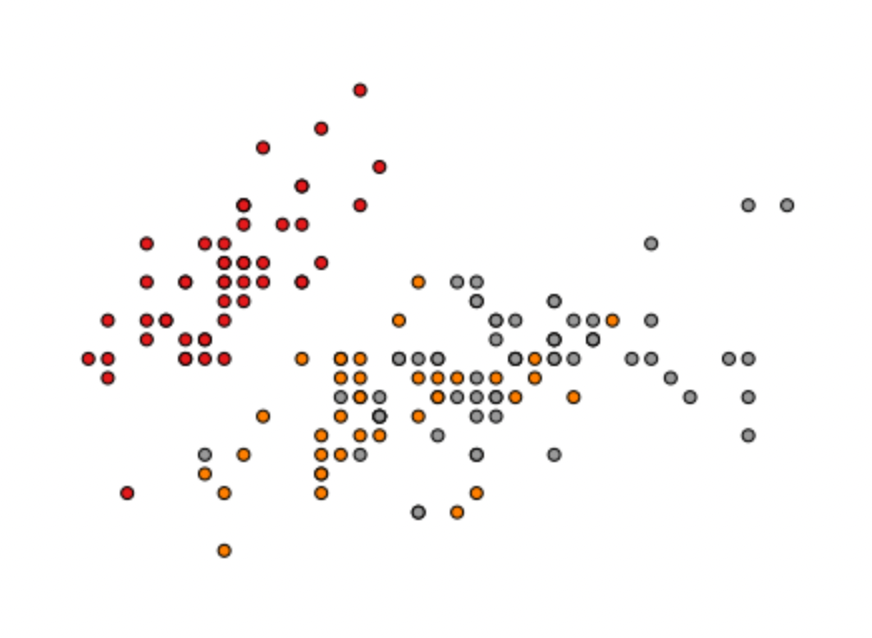
\includegraphics[width=6cm]{images/img5.png}
    \caption{\label{img5}Distribuição dos dados}
  \end{figure}

Uma rede RBF foi treinada com 3 clusters e valores de lâmbida variando de 0.1 a 1.
Para cada valor de lâmbida foi calculado o somatório do erro quadrático de predição e a norma quadrática dos pesos de treinamento w.

\begin{figure}[H]
    \center
    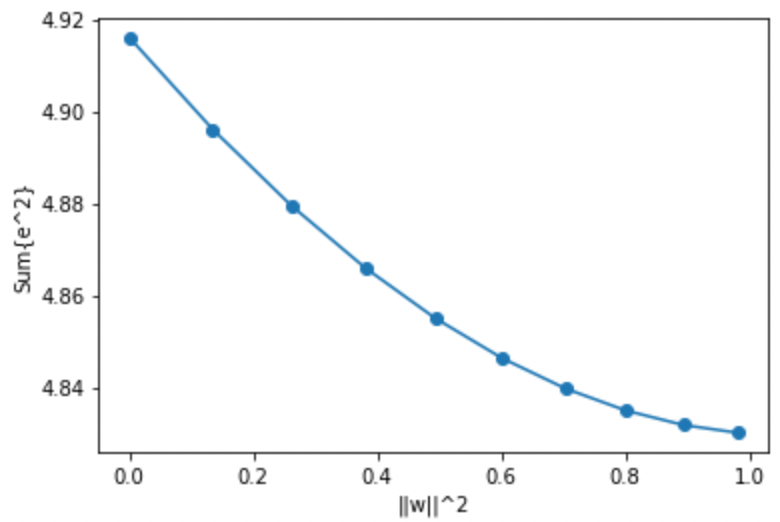
\includegraphics[width=7cm]{images/img6.png}
    \caption{\label{img6}Conjunto de soluções regularizadas}
\end{figure}

Podemos ver a curva de soluções Pareto-Ótimas na figura \ref*{img6}



\subsection*{Experimento 3}

A base de dados utilizada nesse experimento foi a Breast Cancer disponibilizada na biblioteca sklearn. Essa base de dados tem por finalidade
prever se um paciente apresenta sinais de câncer de mama de acordo com o resultado de diversos exames.

Para esse experimento foi analisado a acurácia média de previsão do algoritmo para diversos valores de lâmbida na regularização de uma rede neural RBF.
O resultado está explicitado na figura \ref*{img7}

\begin{figure}[H]
    \center
    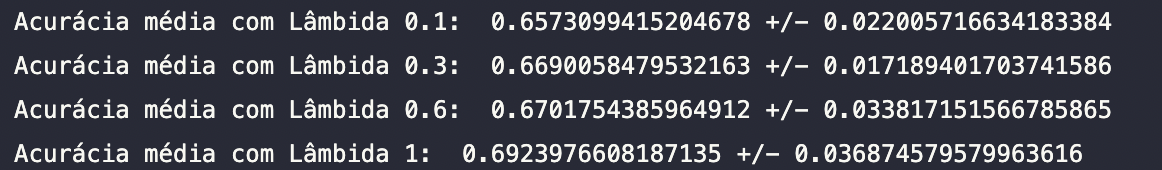
\includegraphics[width=8cm]{images/img7.png}
    \caption{\label{img7}Acurácia da rede RBF regularizada no dataset Breast Cancer}
\end{figure}




\subsection*{Experimento 4}

Por fim, foi implementado o mesmo teste realizado no experimento 2, porém com o dataset Breast Cancer.
Podemos ver na figura \ref*{img8} que a curva de soluções não apresentou uma característica de decaimento semelhante ao da figura \ref*{img6}.

\begin{figure}[H]
    \center
    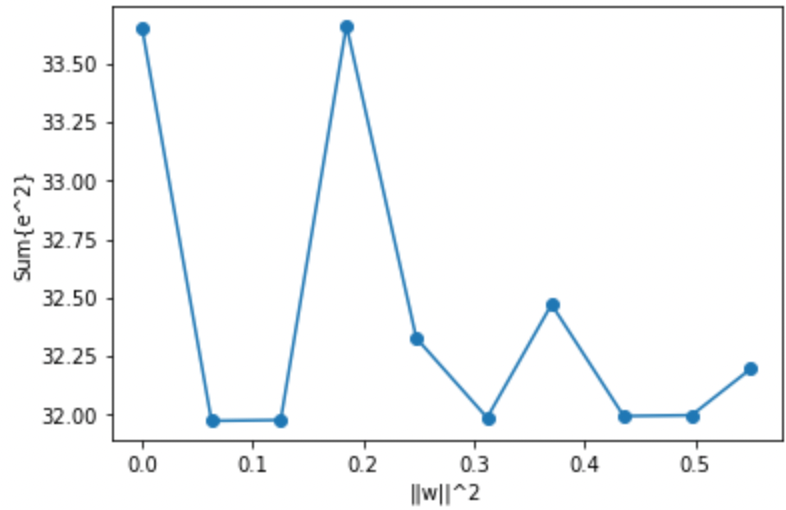
\includegraphics[width=6cm]{images/img8.png}
    \caption{\label{img8}Soluções de uma rede RBF regularizada com dataset Breast Cancer}
\end{figure}